\documentclass{article}
\usepackage[pdftex]{graphicx}
\usepackage{amsmath}
\usepackage{verbatim}
\usepackage{enumerate}
\author{Michael Anderson}
\title{Homework 2}
\begin{document}
\maketitle
\center{CS534}
\center{Prof. Fern}\\
\flushleft
\newpage

\section{}
\begin{enumerate}[(a)]
\item
Decision boundaries for the given tree:

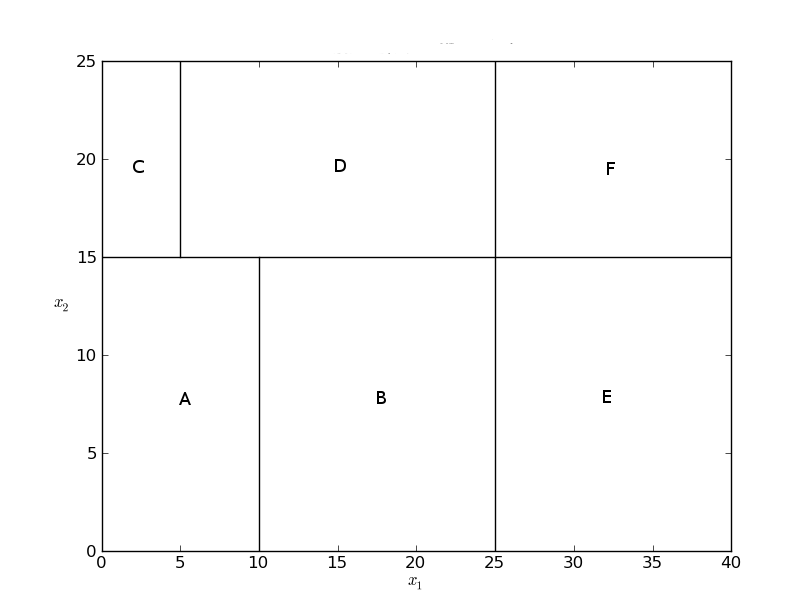
\includegraphics[scale=0.5]{prob1a.png}

\item
Different tree for same set of boundaries:

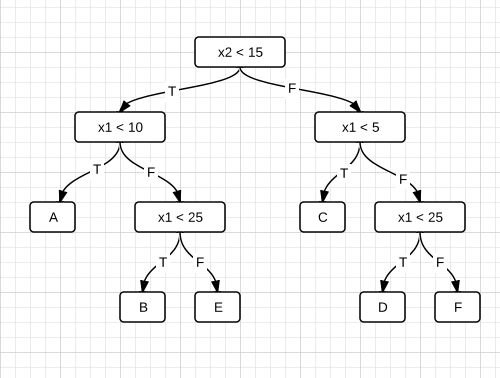
\includegraphics[scale=0.65]{prob1b.png}

The syntactic redundancy is a computational problem, because it creates a
larger search space of possible trees. We do not get anything extra of value
from the larger search space, just more possibilities to wade through until
we find a correct tree for the correct decision boundary. 
\end{enumerate}

\section{}
\begin{enumerate}[(a)]
\item
Suppose that some split about a feature value $X_n=x$ sends
no training examples to one of its children. This means it sends all of its
training examples to the other child. In terms of splitting up the examples, we
are back where we started when we go to split the child with all of the training
examples, and so this is equivalent to saying that the
split did not decrease our uncertainty about Y, and that 
$H(Y) - H(Y|X_n=x) = 0$.

\vspace{1em}

Since $I(Y;X_n=x) = H(Y) - H(Y|X_n=x)$, this further implies that the mutual
information between the two variables is 0. Iff a split about a feature
sends no training examples to one of its children, the feature has 0 mutual
information with the training set; so a split about a feature that has non-zero
mutual information with the training set must send at least one training
example to each of its children.

\item
It is possible that each split could assign one training example to one child,
and the remaining training examples to the other child, which would create a
decision class for each training example. So there could be as many as $m$ leaf
nodes.

\item
It seems that here as well the upper bound is $m$, but I'm honestly
not really sure how to compute this.

\item
According to my guess, the leaf nodes of both are upper bounded by $m$. It seems
plausible that the maximum mutual information tree could have an upper bound
$< m$. If that is the case, then the maximum mutual information tree would
be more accurate because there would be fewer classification bins used to
classify the training data, and a smaller chance of overfitting the data with
more bins that are no more accurate.

\end{enumerate}

\section{}
\begin{enumerate}[(a)]
\item

$P(Y = 0) = 1/2$ \\
$P(A = 0 | Y = 0) = 2/3$ \\
$P(B = 0 | Y = 0) = 1/3$ \\
$P(C = 0 | Y = 0) = 1/3$ \\

\vspace{6pt}

In this particular example 0 and 1 occur equally often in each of the four
variables, so I do not need to count any further.

\vspace{6pt}

$P(Y = 0| (A=0,B=0,C=0)) = 0.5 * 2/3 * 1/3 * 1/3$
$P(Y = 1| (A=0,B=0,C=0)) = 0.5 * 1/3 * 2/3 * 2/3$
$P(Y = 0| (A=0,B=0,C=1)) = 0.5 * 2/3 * 1/3 * 2/3$
$P(Y = 1| (A=0,B=0,C=1)) = 0.5 * 1/3 * 2/3 * 1/3$
$P(Y = 0| (A=0,B=1,C=0)) = 0.5 * 2/3 * 2/3 * 1/3$
$P(Y = 1| (A=0,B=1,C=0)) = 0.5 * 1/3 * 2/3 * 2/3$
$P(Y = 0| (A=0,B=1,C=1)) = 0.5 * 2/3 * 2/3 * 2/3$
$P(Y = 1| (A=0,B=1,C=1)) = 0.5 * 1/3 * 2/3 * 1/3$
$P(Y = 0| (A=1,B=0,C=0)) = 0.5 * 1/3 * 1/3 * 1/3$
$P(Y = 1| (A=1,B=0,C=0)) = 0.5 * 2/3 * 2/3 * 2/3$
$P(Y = 0| (A=1,B=0,C=1)) = 0.5 * 1/3 * 1/3 * 2/3$
$P(Y = 1| (A=1,B=0,C=1)) = 0.5 * 2/3 * 2/3 * 1/3$
$P(Y = 0| (A=1,B=1,C=0)) = 0.5 * 1/3 * 2/3 * 1/3$
$P(Y = 1| (A=1,B=1,C=0)) = 0.5 * 2/3 * 2/3 * 2/3$
$P(Y = 0| (A=1,B=1,C=1)) = 0.5 * 1/3 * 2/3 * 2/3$
$P(Y = 1| (A=1,B=1,C=1)) = 0.5 * 2/3 * 2/3 * 1/3$

\vspace{6pt}

For (A = 1, B = 0, C = 0) predict Y = 1, because $0.5(2/3)^3 > 0.5(1/3)^3$.

\item
Yes, because saying that two random variables are independent is strictly
stronger than saying that they are conditionally independent. If A and B are
not conditionally independent over Y, then they cannot be independent because
knowing the value of one would influence the value of the other through the
relationship they share with Y.

\item
We have that the feature $X_k$ chosen at each split is given by minimizing the
entropy of $(Y|X_k)$, where $Y$ is the set of training examples given to the
node to split. In other words:

\[
X_k = \underset{X}{\operatorname{argmax}}
[-\sum_x P(X_i = x) \sum_y P(Y = y | X_i = x) \log P(Y = y | X_i = x)]
\]

For the data given:

\[
H(Y|A) = H(Y|C) = -\frac{1}{2}[\frac{2}{3} log(\frac{2}{3})
+ \frac{1}{3} log(\frac{1}{3})] - 
\frac{1}{2}[\frac{1}{3} log(\frac{1}{3})
+ \frac{2}{3} log(\frac{2}{3})] \approx .63
\]

\[
H(Y|B) = -\frac{1}{3}[\frac{1}{2} log(\frac{1}{2})
+ \frac{1}{2} log(\frac{1}{2})] - 
\frac{2}{3}[\frac{1}{3} log(\frac{1}{3})
+ \frac{2}{3} log(\frac{2}{3})] \approx .69
\]


$H(Y|A) = H(Y|C)$ and $H(Y|A) < H(Y|B)$, There is a tie between a split about
$A$ and $C$. I will arbitrarily choose a split about $A$.

\vspace{1em}

If $A = 0$:

\[
H(Y|B) = -\frac{1}{3}[0 + 0] - 
\frac{2}{3}[\frac{1}{2} log(\frac{1}{2})
+ \frac{1}{2} log(\frac{1}{2})]
\]

\[
H(Y|C) = -\frac{2}{3}[\frac{1}{2} log(\frac{1}{2})] - 
\frac{1}{3}[0+0]
\]

Here again the two values are completely equal, so arbitrarily split about B

\vspace{1em}

Now by looking at the data we see that if $A = 0$ and $B = 0$ predict 0. If
$A = 0$ and $B = 1$ then predict $\neg C$.

\vspace{1em}

Still have to handle $A = 1$. Since I'm practiced at this by this point, can
see from the data that $H(Y|B) = H(Y|C)$, so arbitrarily split about B.

\vspace{1em}

Now by looking at the data we see that if $A = 1$ and $B = 0$ predict 1. If
$A = 1$ and $B = 1$ then predict $\neg C$. So here's what the final tree looks
like:

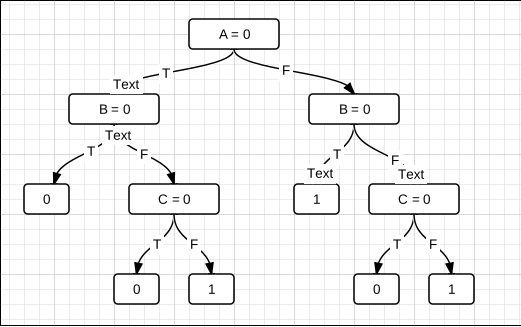
\includegraphics[scale=0.65]{prob3c.png}

\end{enumerate}

\section{}
\begin{enumerate}[(a)]
\item
\[
\hat{y} = \sigma(W_i \cdot A^T) = \frac{e^{x_i}}{\sum_{j=1}^{3}e^{x_j}}
(W_i \cdot A_T)
\]

\[
J(w) = \frac{1}{2}\sum_{i=1}^N(\frac{e^{x_i}}{\sum_{j=1}^{3}e^{x_j}}
(W_i \cdot A_T) - y_i)^2
\]

\item
\[
\frac{\partial J(w)}{\partial w_{9,6}} =
(\hat y_i - y) \cdot \frac{\partial}{\partial w_{9,6}}
(\sigma(W_9 \cdot A^T) - y_i)
\]

\item
\[
\frac{\partial J(w)}{\partial w_{6,3}} =
(\hat y_i - y) \cdot \frac{\partial}{\partial w_{6,3}}
(\sigma(W_6 \cdot X^T) - y_i)
\]

\item
\begin{verbatim}
epsilon <- acceptable level of error
while error > epsilon
    error = 0
    for each training example y:
        error <- error + (yHat - y)
    for each output node v:
        for each hidden node u:
            w(v,u) <- w(v,u) - nu[error([sigma]W(v)A^T) - y(i)]'
    for each hidden node j:
        w(j,v) <- w(j,v) - nu[delta(u)x(i,j)]
do until error < epsilon
\end{verbatim} 

\end{enumerate}
\section{}
\[
(x^i + x^j + 1)^3 = (x^i + x^j + 1)^2(x^i + x^j + 1) =
\]

\[
(x^{i^2}_1x^{j^2}_1 + 2x^i_1x^i_2x^j_1x^j_2+x^{i^2}_2 x^{j^2}_2+ 2x^i_1x^j_1 
+ 2x^i_2x^j_2 +1)(x^i + x^j + 1) =
\]

\[
x^{i^3}_1x^{j^3}_1 + 3x^{i^2}_1 x^i_2 x^{j^2}_1 x^j_2 + 3x^{i^2}_1x^{j^2}_1 +
3x^i_1 x^{i^2}_2 x^j_1 x^{j^2}_2 + 6 x^i_1 x^i_2 x^j_1 x^j_2 + 3 x^i_1 x^j_1
+ x^{i^3}_2x^{j^3}_2 + 3x^{i^2}_2x^{j^2}_2 + 3 x^i_2 x^j_2 + 1 = 
\]

\[
(x^{i^3}_1, \sqrt{3}x^{i^2}_1 x^i_2, \sqrt{3}x^{i^2}_1,
\sqrt{3}x^i_1 x^{i^2}_2, \sqrt{6} x^i_1 x^i_2, \sqrt{3} x^i_1,
x^{i^3}_2, \sqrt{3}x^{i^2}_2, \sqrt{3} x^i_2, 1) +
\]

\[
(x^{j^3}_1, \sqrt{3}x^{j^2}_1 x^j_2, \sqrt{3}x^{j^2}_1,
\sqrt{3}x^j_1 x^{j^2}_2, \sqrt{6} x^j_1 x^j_2, \sqrt{3} x^j_1,
x^{j^3}_2, \sqrt{3}x^{j^2}_2, \sqrt{3} x^j_2, 1) = 
\]

\[
\phi(x^i) \cdot \phi(x^j)
\]

\end{document}
